\documentclass[a4paper]{article}
\addtolength{\hoffset}
{-2.25cm}
\addtolength{\textwidth}
{5cm}
\addtolength{\voffset}
{-3.25cm}
\addtolength{\textheight}
{5.5cm}
\setlength{\parskip}{0pt}
\setlength{\parindent}{0in}

\usepackage[utf8]{inputenc}
\usepackage{microtype}
\usepackage[english]{babel}
\usepackage{fancyhdr}
\usepackage{advdate}
\usepackage{enumitem}
\usepackage{amsmath, amssymb}
\usepackage{graphicx}
\usepackage{caption}
\usepackage{subcaption}
\usepackage{float}
\usepackage{titlesec}
\usepackage{wasysym}
\usepackage{url}
\usepackage{hyperref}
\usepackage{tikz, verbatimbox}
\usepackage{fixltx2e}
\usepackage{centernot}
\usepackage{algorithm}
\usepackage{algpseudocode}
\usepackage{listings}
\usetikzlibrary{shapes.geometric, arrows}
\usetikzlibrary{positioning}
\usepackage[table]{xcolor}

\graphicspath{{./static/}}
\tikzset{every picture/.style={line width=0.75pt}} %set default line width to 0.75pt

\newcommand{\LComment}[1]{\State \(\triangleright\) \text{#1}}
\MakeRobust{\Call}
\usepackage{pdfpages}

\begin{document}

\fancyhead[c]{}
\hrule \medskip
\begin{minipage}{0.295\textwidth}
\raggedright
Rishabh Indoria\\
21F3001823
\end{minipage}
\begin{minipage}{0.4\textwidth}
\centering
\LARGE
Deep Learning
\end{minipage}
\begin{minipage}{0.295\textwidth}
\raggedleft
\today \hfill \\
\end{minipage}
\medskip \hrule
\bigskip

\section{History of Deep Learning}

\subsection{Biological Neurons}
\begin{itemize}
    \item \textbf{Reticular Theory}: Nervous system is a single continuous network as opposed to a network of many discrete cells.
    \item \textbf{Staining Technique}: Chemical reaction that allows to examine nervous tissue in much greater detail.
    \item \textbf{Neuron Doctrine}: Nervous system is actually made up of discrete individual cells forming a network.
\end{itemize}
\subsection{From Spring to Winter of AI}
\begin{itemize}
    \item \textbf{McCulloch Pitts Neuron}: A highly simplified model of the neuron.
    \item \textbf{Perceptron}: "The perceptron may eventually be able to learn, make decisions, and translate languages."
    \item "The embryo of an electric computer that the Navy expects will be able to walk, talk, see, write, reproduce itself and be conscious of its existence."
    \item Book "\textbf{Perceptrons}" by Minsky and Papert outlined the limits of what perceptrons could do.
    \item \textbf{Backpropagation}: First used in the context of artificial neural networks.
    \item \textbf{Universal Approximation Theorem}: A multilayered network of neurons with a single hidden layer can be used to approximate any continuous function to any desired precision.
    \begin{figure}[H]
        \centering
        \begin{subfigure}[b]{0.45\textwidth}
             \centering
             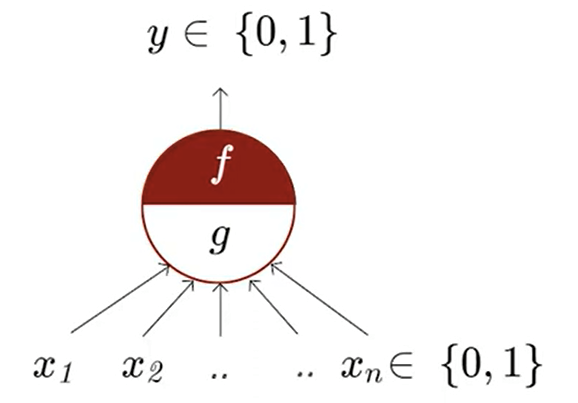
\includegraphics[width=\textwidth]{Degree/static/DL_simple_neuron.png}
             \caption{Simple Model of the Neuron}
             \label{fig:DL-simple-neuron}
         \end{subfigure}
         \hfill
        \begin{subfigure}[b]{0.45\textwidth}
            \centering
            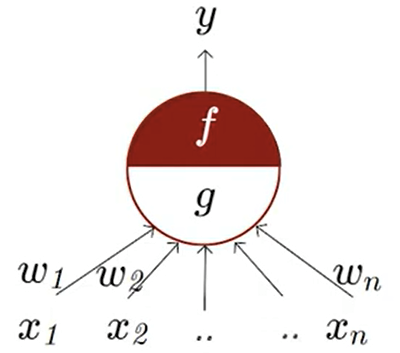
\includegraphics[width=0.71\textwidth]{Degree/static/DL_perceptron.png}
            \caption{Model of the Perceptron}
            \label{fig:DL-perceptron}
        \end{subfigure}
        \caption{First models of neurons}
        \label{fig:DL-first-neurons}
    \end{figure}
\end{itemize}

\subsection{The Deep Revival}
\begin{itemize}
    \item \textbf{Unsupervised Pre-Training}: Described an effective way of initializing the weights that allows deep autoencoders networks to learn a low-dimensional representation of data.
\end{itemize}

\subsection{From Cats to Convolutional Neural Networks}
\begin{itemize}
    \item \textbf{Hubel and Wiesel Experiment}: Experimentally showed that each neuron has a fixed receptive field -i.e. a neuron will fire only in response to visual stimuli in a  specific region in the visual space(Motivation for CNNs).
\end{itemize}

\subsection{Faster, higher, stronger}
\begin{itemize}
    \item \textbf{Better Optimization Methods}: Faster convergence, better accuracies. Examples: AdaGrad, RMSProp, Adam, Nadam, etc.
    \item \textbf{Better Activation Functions}: Many new functions have been proposed, leading to better convergence and performance. Example: tanh, ReLu, Leaky Relu, etc.
\end{itemize}

\subsection{The Curios Case of Sequences}
\begin{itemize}
    \item \textbf{Sequences}: Each unit in the sequence interacts with other units. Need models to capture this interaction. Example: Speech, Videos, etc.
    \item \textbf{Hopfield Network}: Content-addressable memory systems for storing and retrieving patterns.
    \item \textbf{Jordan Network}: The output state of each time step is fed to the next time step, thereby allowing interactions between time steps in the sequence.
    \item \textbf{Elman Network}: The hidden state of each time step is fed to the next time step, thereby allowing interactions between time steps in the sequence.
    \item Very hard to train RNNs.
    \item \textbf{Long Short Term Memory}: Solve complex long time lag tasks that could never be solved before(solved the problem of vanishing gradient).
    \item \textbf{Sequence to Sequence Models}: Introduction to Attention!!, However, they were unable to capture the contextual information of a sentence.
    \item \textbf{Transformers}: Introduced a paradigm shift in the field of NLP. GPT and BERT are the most commonly used transformer based architectures.
\end{itemize}

\subsection{Beating humans at their own game}
\begin{itemize}
    \item Human-level control through deep reinforcement learning for playing Atari Game
    \item \textbf{OpenAI Gym}: Toolkit for developing and comprising reinforcement learning algorithms. It supports teaching agents everything from walking to playing games like Pong or Pinball.
    \item \textbf{OpenAI Gym Retro}: A platform for reinforcement learning research on games, which contains 1,000 games across a variety of backing emulators.
    \item \textbf{MuZero}: Masters Go, chess, shogi and Atari without needing to be told the rules, thanks to its ability to plan winning strategies in unknown environments.
    \item \textbf{Player of Games(PoG)}: A general purpose algorithm that unifies all previous approached. Learn to play under both perfect and imperfect information games.
\end{itemize}

\subsection{The rise of Transformers}
\begin{itemize}
    \item \textbf{Rule Based Systems}: Initial Machine Translation Systems used handcrafted rules and dictionaries to translate sentences between few politically important language pairs.
    \item \textbf{Statistical MT}: The IBM Models for Machine Translation gave a boost to the idea of data driven statistical NLP, probability based models.
    \item \textbf{Neural MT}: The introduction of seq2seq models and attention. Bigger, hungrier, better models.
    \item \textbf{From Language to Vision}: A vision model based as closely as possible on the Transformer architecture, originally designed for text-based tasks.
    \item \textbf{From Discrimination to Generation}: Sample(Generate) data from the learned probability distribution.Variable Auto Encoders(VAE), Generational Adversarial Networks(GAN), Flow-based models to achieve it.
    \item GANs don't scale, are unstable and capture less diversity. Diffusion models are one of the alternatives to GAN. Inspired by an idea from non-equilibrium thermodynamics.
\end{itemize}

\subsection{Call for Sanity}
\begin{itemize}
    \item \textbf{Paradox of Deep Learning}: Deep learning works so well despite high capacity(susceptible to overfitting), numerical instability(vanishing/exploding gradients), sharp minima(leads to overfitting), non-robustness.
    \item \textbf{Interpretable Machine Learning: A Guide for Making Black Box Models Explainable} by Christoph Molnar.
    \item \textbf{AI Audit challenge}: AI systems must be evaluated for legal compliance, in particular laws protecting people from illegal discrimination. This challenge seeks to broaden the tools available to people who want to analyze and regulate them.
    \item \textbf{Analog AI}: Programmable resistors are the key building blocks in analog deep learning, just like transistors are the core element of digital processors(faster computation).
\end{itemize}

\subsection{The AI revolution in basic Science Research}
\begin{itemize}
    \item \textbf{Protein-Folding Problem}: Model proposed to predict protein structure, which would lead to better drug development.
    \item \textbf{Astronomy: Galaxy Evolution}: Predict how galaxies would look like as it gets older.
\end{itemize}

\subsection{Efficient Deep Learning}

\begin{itemize}
    \item Build models on small devices, aka phones. Deploying models in resource-constrained devices.
\end{itemize}

\section{Multi Layered Network of Perceptrons}
\subsection{Biological Neurons}
\begin{itemize}
    \item The most fundamental unit of a deep neural network is called an artificial neuron.
    \item The inspiration comes from biology(more specifically, from the brain).
    \item \textbf{biological neurons = neural cells = neural processing units}
    \item \textbf{Dendrite}: Receives signals from other neurons\\
    \textbf{Synapse}: Point of connection to other neurons\\
    \textbf{Soma}: Processes the information\\
    \textbf{Axon}: Transmits the output of this neuron.
    \item This massively parallel network also ensures that there is division of work. Each neuron may perform a certain role or respond to a certain stimulus. The neurons in the brain arranged in a hierarchy.
    \begin{figure}[H]
        \centering
        \begin{subfigure}[b]{0.3\textwidth}
            \centering
            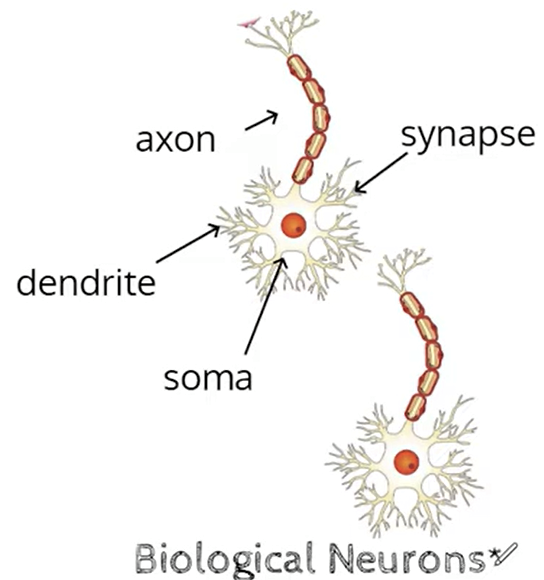
\includegraphics[width=0.9\textwidth]{Degree/static/DL_biological_neuron.png}
            \caption{Biological Neuron}
            \label{fig:DL-biological-neuron}
        \end{subfigure}
        \begin{subfigure}[b]{0.3\textwidth}
            \centering
            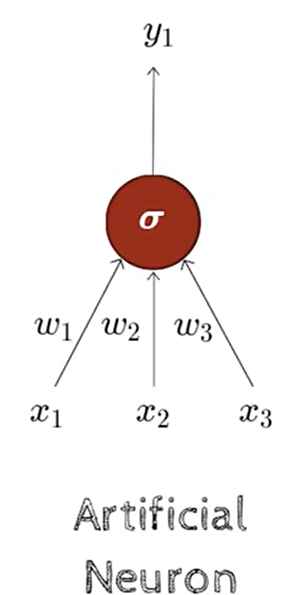
\includegraphics[width=0.5\textwidth]{Degree/static/DL_artificial_neuron.png}
            \caption{Artificial Neuron}
            \label{fig:DL-artificial-neuron}
        \end{subfigure}
        \begin{subfigure}[b]{0.3\textwidth}
            \centering
            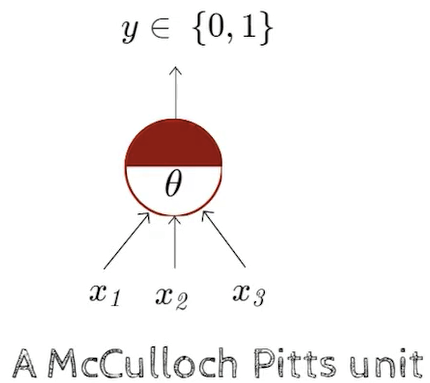
\includegraphics[width=\textwidth]{Degree/static/DL_Pitts_unit.png}
            \caption{A McCulloch Pitts Unit}
            \label{fig:DL-pitts-neuron}
        \end{subfigure}
        \caption{Basic Neuron Structure}
        \label{fig:DL-basic-neurons}
    \end{figure}
    \item \textbf{McCulloch Pitts Neuron}: Proposed a highly simplified computational model of the neuron. $g$ aggregates the inputs, and the function $f$ takes a decision based on this aggregation. The inputs can be excitatory or inhibitory.\\
    \textbf{Example}: $y=0$ if any $x_i$ is inhibitory, else $g(x_1,...,x_n)=g(x)=\sum_{i=1}^nx_i$\\
    $y=f(g(x))=1$ if $g(x)\geq \theta$ else $0$\\
    $\theta$ is called the thresholding parameter.
    \item circle at the end indicates inhibitory input if any inhibitory input is $1$ then the output will be $0$.
    \item Linear separability(for boolean functions): There exists a line(plane) such that all inputs which produce a $1$ lie on one side of the line(plane) and all inputs which produce a $0$ lie on the other side of the line(plane).
    \item A single McCulloch Pitts Neuron can be used to represent boolean functions which are linearly separable.
    \item It can be trivially seen that $\theta=0$ for the Tautology(always ON) function.
    \begin{figure}[H]
        \centering
        \begin{subfigure}[b]{0.225\textwidth}
            \centering
            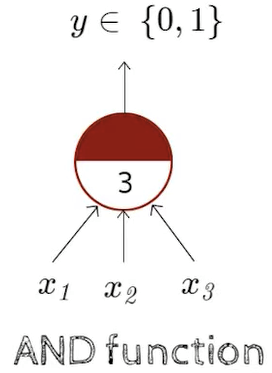
\includegraphics[width=1\textwidth]{Degree//static/DL_Pitts_AND.png}
            \caption{AND function}
            \label{fig:DL-pitts-AND}
        \end{subfigure}
        \hfill
        \begin{subfigure}[b]{0.225\textwidth}
            \centering
            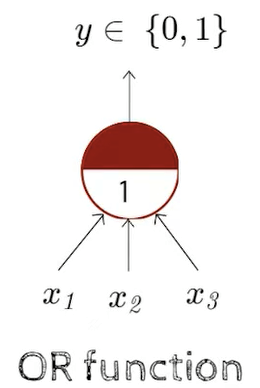
\includegraphics[width=0.9\textwidth]{Degree//static/DL_Pitts_OR.png}
            \caption{OR function}
            \label{fig:DL-pitts-OR}
        \end{subfigure}
        \hfill
        \begin{subfigure}[b]{0.225\textwidth}
            \centering
            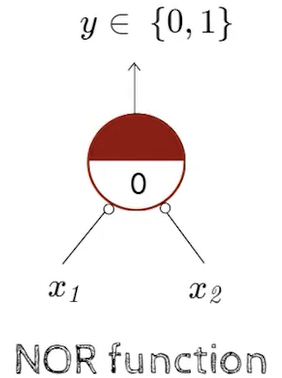
\includegraphics[width=1\textwidth]{Degree//static/DL_Pitts_NOR.png}
            \caption{NOR function}
            \label{fig:DL-pitts-NOR}
        \end{subfigure}
        \hfill
        \begin{subfigure}[b]{0.225\textwidth}
            \centering
            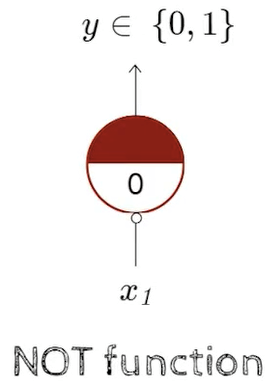
\includegraphics[width=1\textwidth]{Degree//static/DL_Pitts_NOT.png}
            \caption{NOT function}
            \label{fig:DL-pitts-NOT}
        \end{subfigure}
        \caption{Basic Boolean functions}
        \label{fig:DL-basic-boolean}
    \end{figure}
\end{itemize}

\subsection{Perceptrons}
\begin{itemize}
    \item \textbf{Classical Perceptron}: Frank Rosenblatt proposed this model, which was refined and carefully analyzed by Minsky and Papert.
    \item Main difference is the introduction of numerical weights for inputs and a mechanism for learning these weights.
    \item $y=1$ \textit{if} $\sum_{i=1}^nw_i\times x_i \geq \theta$ else $0$.\\
    If we take $\theta$ on one side and represent $w_0=-\theta$ and $x_0=1$, then we have\\
    $y=1$ \textit{if} $\sum_{i=0}^nw_i\times x_i\geq 0$ else $0$.
    \item $w_0$ is called the bias as it represents the \textbf{prior}(prejudice).
    \item From the equation, it can be clearly seen that a perceptron separates the input space into two halves. A single perceptron can only be used to implement linearly separable functions.
    \item The difference between this and the MP neuron is that now we have weights that can be learned, and the inputs can be real values.
    \begin{figure}[H]
        \centering
        \begin{subfigure}[b]{0.45\textwidth}
            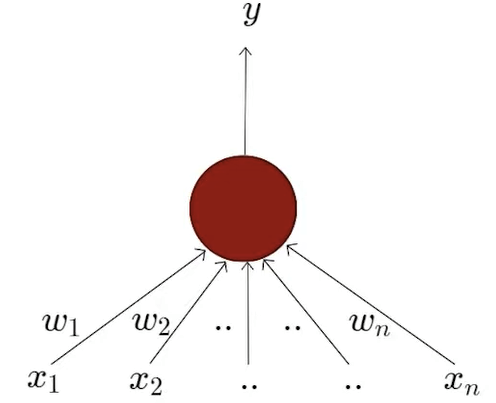
\includegraphics[width=0.8\textwidth]{Degree//static/DL_classical_perceptron.png}
            \caption{Perceptron}
            \label{fig:DL-perceptron}
        \end{subfigure}
        \hfill
        \begin{subfigure}[b]{0.45\textwidth}
            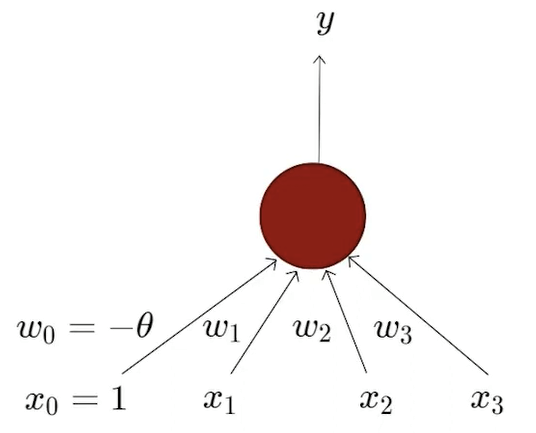
\includegraphics[width=0.8\textwidth]{Degree/static/DL_perceptron_bias.png}
            \caption{Perceptron with $w_0$}
            \label{fig:DL-perceptron-bias}
        \end{subfigure}
        \caption{Classical Perceptrons}
        \label{fig:DL-classical-perceptrons}
    \end{figure}
\end{itemize}

\subsection{Perceptron Learning Algorithm}
\begin{itemize}
    \item \textbf{Perceptron learning algorithm}: Consider two vectors $w=[w_0,...,w_n]$ and $x=[1,x_1,...,x_n]$, then $w\times x=w^Tx$ or the dot product. We can rewrite the perceptron rule as $y=1$ \textit{if} $w^Tx\geq 0$ else $0$.\\
    \item We are interested in finding the line $w^Tx=0$ which divides the input space into two halves. The angle $\alpha$ between $w$ and any point $x$ which lies on the line must be $90^{\circ}$ because $\cos{\alpha}=\frac{w^Tx}{||w||||x||}=0$. So, the vector $w$ is perpendicular to every point on the line, then it is perpendicular to the line itself.
    \item For any point such that $w^Tx>0$ we will have $\alpha<90^{\circ}$ and for any point such that $w^Tx<0$ we will have $\alpha>90^{\circ}$.
    \begin{algorithm}[H]
        \caption{Perceptron Learning Algorithm}\label{alg:DL-perceptron-learning-alg}
        \begin{algorithmic}[1]
            \State $P\gets$ \textit{inputs with label }$1$;
            \State $N\gets$ \textit{inputs with label }$0$;
            \State Initialize \textbf{w} randomly
            \While{!\textit{convergence}}
                \State Pick random $x\in P\cup N$;
                \If{$x\in P$ \textit{and} $\sum_{i=0}^nw_i\times x_i<0$}
                    \State \textbf{w} = \textbf{w} + \textbf{x};
                \EndIf
                \If{$x\in N$ \textit{and} $\sum_{i=0}^nw_i\times x_i\geq 0$}
                    \State \textbf{w} = \textbf{w} - \textbf{x};
                \EndIf
            \EndWhile
            \LComment{the algorithm converges when all the inputs are classified correctly}
        \end{algorithmic}
    \end{algorithm}
    \item For $x\in P$ if $w^Tx<0$ then it means that the angle $\alpha$ between this $x$ and the current $w$ is greater than $90^{\circ}$, but we want it to be $<90^{\circ}$.\\
    When we do $w_{new}=w+x$, alpha changes as follows
    \begin{equation*}
        \cos{\alpha_{new}}\propto (w_{new}^Tx)=(w+x)^Tx=W^Tx+x^Tx=\cos{\alpha}+x^Tx
    \end{equation*}
    \begin{equation*}
        \cos{\alpha_{new}}>\cos{\alpha}\implies \alpha_{new}<\alpha
    \end{equation*}
    $\alpha_{new}$ becomes less than, $\alpha$ which is exactly what we wanted, we may not get $<90^{\circ}$ in one shot so we keep doing it. Similarly, it can be shown for $x\in N$.
    \item \textbf{Definition}: Two sets $P$ and $N$ of points in an $n-$dimensional space are called absolutely linearly separable if $n+1$ real numbers $w_0,...,w_n$ exist such that every point $(x_1,...,x_n)\in P$ satisfies $\sum_{i=1}^nw_i\times x_i\geq w_0$ and every point $(x_1,...,x_n)\in N$ satisfies $\sum_{i=1}^nw_i\times x_i<w_0$.
    \item \textbf{Proposition}: If the sets $P$ and $N$ are finite and linearly separable, the perceptron learning algorithm updates the weight vector $w$ a finite number of times. In other words: if the vectors in $P$ and $N$ are tested cyclically one after the other, a weight vector $w$ is found after a finite number of steps $t$ which can separate the two sets.
    \item \textbf{Proof of Convergence}: If $x\in N$, then $-x\in P$ ($\therefore w^Tx<0\implies w^T(-x)\geq 0$).\\
    We can now consider only a single set $P'=P\cup N^-$ and for every element $p\in P'$ ensure that $w^Tp\geq 0$.
    \begin{algorithm}[H]
        \caption{Modified Perceptron Learning Algorithm}\label{alg:DL-modified-perceptron-learning-alg}
        \begin{algorithmic}[1]
            \State $P\gets$ \textit{inputs with label }$1$;
            \State $N\gets$ \textit{inputs with label }$0$;
            \State $N^-\gets$ \textit{negations of all points in }$N$;
            \State $P'\gets P\cup N^-$
            \State Initialize \textbf{w} randomly
            \While{!\textit{convergence}}
                \State Pick random $p\in P'$;
                \If{$\sum_{i=0}^nw_i\times p_i<0$}
                    \State \textbf{w} = \textbf{w} + \textbf{p};
                \EndIf
            \EndWhile
            \LComment{the algorithm converges when all the inputs are classified correctly}
        \end{algorithmic}
    \end{algorithm}
    Further we will normalize all the $p$'s so that $||p||=1$, notice this does not change anything in our step.\\
    Let $w^*$ be the normalized solution vector(we know one exists whose value we don't know).\\
    Now suppose at some time step $t$ we inspected the point $p_i$ and found that $w^Tp_i<0$, then we make correction $w_{t+1}=w_t+p_i$.\\
    Let $\beta$ be the angle between $w^*$ abd $w_{t+1}$, then we have $\cos{\beta}=\frac{w^*w_{t+1}}{||w_{t+1}||}$
    \begin{equation*}
    \begin{split}
        Numerator\text{ }=w^*\cdot w_{t+1}=x^*\cdot (w_t+p_i)=w^*\cdot w_{t} + w^*\cdot p_i\geq w^*\cdot w_{t}+\delta \text{ }(\delta=\min(w^*\cdot p_i|\forall i))\\
        \geq w^*\cdot(w_{t-1}+p_j)+\delta \geq w^*\cdot w_{t-1} + w^*\cdot p_j + \delta \geq w^*\cdot w_{t-1}+2\delta \geq w^*w_0+(k)\delta \text{ }(By\text{ }Induction)
    \end{split}
    \end{equation*}
    \begin{equation*}
    \begin{split}
        Denominator^2\text{ }=||w_{t+1}||^2=(w_{t}+p_i)\cdot(w_{t}+p_i)=||w_t||^2+2w_t\cdot p_i+||p_i||^2\leq ||w_t||^2+||p_i||^2\\
        \leq ||w_t||^2+1\leq (||w_{t-1}||^2+1)+1\leq ||w_0||^2+(k)
    \end{split}
    \end{equation*}
    So, we have $Numerator\geq w^*\cdot w_0+(k)\delta$ and $Denominator^2\leq ||w_0||^2+(k)$
    \begin{equation*}
        \cos{\beta}\geq \frac{w^*\cdot w_0+k\delta}{\sqrt{||w_0||^2+k}}
    \end{equation*}
    $\cos{\beta}$ grows proportional to $\sqrt{k}$\\
    As $k$(number of corrections) increase $\cos{\beta}$ can become arbitrarily large, but since $\cos{\beta}\leq 1$, $k$ must be bounded by a maximum order.\\
    Thus, there can only be a finite number of corrections $(k)$ to $w$ and the algorithm will converge!
\end{itemize}

\subsection{Linearly Separable Boolean Function}
\begin{itemize}
    \item One simple example that is not linearly separable is XOR
    \begin{table}[H]
        \centering
        \begin{tabular}{cccc}
            \hline
            $x_1$ & $x_2$ & XOR &  \\
            \hline
            0 & 0 & 0 & $w_0+\sum_{i=1}^2w_ix_i<0$\\
            1 & 0 & 1 & $w_0+\sum_{i=1}^2w_ix_i\geq0$\\
            0 & 1 & 1 & $w_0+\sum_{i=1}^2w_ix_i\geq0$\\
            1 & 1 & 0 & $w_0+\sum_{i=1}^2w_ix_i<0$\\
            \hline
        \end{tabular}
        \caption{XOR Truth Table}
        \label{tab:DL-XOR-truth}
    \end{table}
    \item Most real world data is not linearly separable and will always contain some \textbf{outliers}.
    \item How many boolean functions can we design from 2 inputs.
    \begin{table}[H]
        \centering
        \begin{tabular}{cccccccccccccccccc}
            \hline
            $x_1$ & $x_2$ & $f_1$ & $f_2$ & $f_3$ & $f_4$ & $f_5$ & $f_6$ & $f_7$ & $f_8$ & $f_9$ & $f_{10}$ & $f_{11}$ & $f_{12}$ & $f_{13}$ & $f_{14}$ & $f_{15}$ & $f_{16}$ \\
            \hline
            0 & 0 & 0 & 0 & 0 & 0 & 0 & 0 & 0 & 0 & 1 & 1 & 1 & 1 & 1 & 1 & 1 & 1\\
            1 & 0 & 0 & 0 & 0 & 0 & 1 & 1 & 1 & 1 & 0 & 0 & 0 & 0 & 1 & 1 & 1 & 1\\
            0 & 1 & 0 & 0 & 1 & 1 & 0 & 0 & 1 & 1 & 0 & 0 & 1 & 1 & 0 & 0 & 1 & 1\\
            1 & 1 & 0 & 1 & 0 & 1 & 0 & 1 & 0 & 1 & 0 & 1 & 0 & 1 & 0 & 1 & 0 & 1\\
            \hline
        \end{tabular}
        \caption{Functions of 2 inputs}
        \label{tab:DL-2-ip-functions}
    \end{table}
    Out of these, only XOR and !XOR are not linearly separable.
    \item In general, we can have $2^{2^n}$ boolean functions in $n$ inputs.
\end{itemize}

\subsection{Representation Power of a Network of Perceptrons}
\begin{itemize}
    \item We will assume True $=+1$ and False $=-1$, we consider 2 inputs and 4 perceptrons with specific weights. The bias of each perceptron is $-2$. Each of these perceptrons is connected to an output perceptron by weights (which need to be learned). The output of this perceptron $(y)$ is the output of this network.
    \begin{figure}[H]
        \centering
        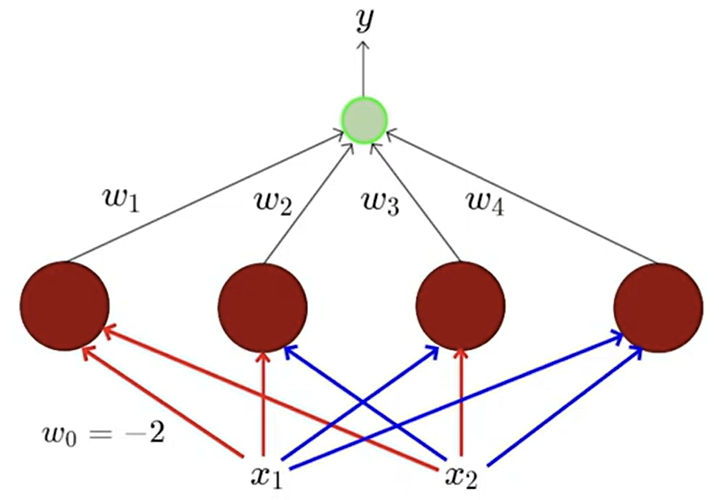
\includegraphics[width=0.5\linewidth]{Degree//static/DL_simple_network.png}
        \caption{Network of Perceptrons}
        \label{fig:DL-simple-network}
    \end{figure}
    red edge indicates $w=-1$, and blue edge indicates $w=+1$. $x_1$ has weights $-1,-1,+1,+1$ and $x_2$ has weights $-1, +1, -1, +1$ from left to right respectively.
    \item The above network contains $3$ layers.\\
    The layer containing the inputs $(x_1,x_2)$ is called the \textbf{input layer}.\\
    The middle layer containing the $4$ perceptrons is called the \textbf{hidden layer}.\\
    The final layer containing one output neuron is called the \textbf{output layer}.\\
    The output of the $4$ perceptrons in the hidden layer are denoted by $h_1,h_2,h_3,h_4$.\\
    The red and blue edges are called layer 1 weights\\
    $w_1,w_2,w_3,w_4$ are called layer 2 weights.
    \item This network can be used to implement \textbf{any} boolean function linearly separable or not. Each perceptron in the middle layer fires only for a specific input and no perceptrons fire for the same input.
    \begin{table}[H]
        \centering
        \begin{tabular}{cccccccc}
            \hline
            $x_1$ & $x_2$ & XOR &  $h_1$ & $h_2$ & $h_3$ & $h_4$ & $\sum_{i=1}^4w_ih_i $\\
            \hline
            0 & 0 & 0 & 1 & 0 & 0 & 0 & $w_1$\\
            1 & 0 & 1 & 0 & 1 & 0 & 0 & $w_2$\\
            0 & 1 & 1 & 0 & 0 & 1 & 0 & $w_3$\\
            1 & 1 & 0 & 0 & 0 & 0 & 1 & $w_4$\\
            \hline
        \end{tabular}
        \caption{Truth Table for the Network}
        \label{tab:DL-network-truth}
    \end{table}
    This results in four independent conditions.
    \item In case of $3$ inputs we would now have $8$ perceptrons in the hidden layer.
    \item \textbf{Theorem}: Any boolean function of $n$ inputs can be represented exactly by a network of perceptrons containing one hidden layer with $2^n$ perceptrons and one output layer containing 1 perceptron.
    \item \textbf{Note}: A network of $2^n+1$ perceptrons is not necessary but sufficient.
    \item \textbf{Catch}: As $n$ increases the number of perceptrons in the hidden layers increases exponentially.
    \item We care about boolean functions, because we can model real world examples into boolean functions or classification problems.
    \item The network we saw is formally known as Multilayer Perceptron(MLP) or more appropriately "Multilayered Network of Perceptrons".
\end{itemize}

\section{Sigmoid Neurons}

\subsection{What are they?}
\begin{itemize}
    \item The thresholding logic used by a perceptron is very harsh! It is a characteristic of the perceptron function itself which behaves like a \textbf{step function}.
    \item For most real world applications we would expect a smoother decision function which gradually changes from 0 to 1.
    \item Instead we would use sigmoid function
    \begin{equation*}
        y=\frac{1}{1+\exp(-(\omega_0+\sum_{i=1}^n\omega_ix_i))}
    \end{equation*}
    \item We no longer see a sharp transition around the threshold $\omega_0$. Also, $y$ now takes any real value in $[0,1]$.
    \item This value can also be interpreted as probability.
\end{itemize}

\subsection{Typical Supervised Machine Learning Setup}\label{sec:DL-typical-ml-setup}
\begin{itemize}
    \item \textbf{Data}: $\{x_i,y_i\}_{i=1}^n$, we have $n$ data point where $x_i$ is a vector of $\mathbb{R}^m$. Assume $y=\hat{f}(x;\theta)$.
    \item \textbf{Model}: Our approximation of the relation between $x$ and $y$.
    \begin{equation*}
        \text{For example, }\hat{y}=\frac{1}{1+e^{-w^Tx}}\text{ or }\hat{y}=w^Tx\text{ or }\hat{y}=x^TWx
    \end{equation*}
    \item \textbf{Learning algorithm}: An algorithm for learning the parameters $w$ of the model.
    \item \textbf{Objective/Loss/Error function}: To guide the learning algorithm. One possibility is $\sum_{i=1}^n(\hat{y}_i-y_i)^2$.
    \item The learning algorithm should aim to minimize the loss function.
\end{itemize}

\subsection{Learning Parameters}
\begin{itemize}
    \item For ease of explanation we will take $f(x)=\frac{1}{1+e^{-(wx+b)}}$, only a single parameter.
    \item Assume input for training data is $\{x_i,y_i\}_{i=1}^N\rightarrow$ $N$ pairs of $(x,y)$.
    \item Training Objective: Find $w$ and $b$ such that $\mathcal{L}(w,b)=\frac{1}{N}\sum_{i=1}^N(y_i-f(x_i))^2$ is minimized.
    \item \textbf{Guess Work(Infeasible)}: Intuitively guess what should be the values of $w$ and $b$. May never end and is not feasible for writing algorithms.
    \item \textbf{Update rule}: $\theta_{new}=\theta + \eta \Delta \theta$, how to find $\Delta \theta$?
    \item \textbf{Taylor Series}: A way of approximating any continuously differentiable function $\mathcal{L}(w)$ using polynomials of degree $n$. The higher the degree the better the approximation!
    \begin{equation*}
        \mathcal{L}(w)=\mathcal{L}(w_0)+\frac{\mathcal{L}'(w_0)}{1!}(w-w_0)+\frac{\mathcal{L}''(w_0)}{2!}(w-w_0)^2+...
    \end{equation*}
    \item Linear approximation is the first order approximation of the Taylor series. Quadratic approximation is the second order approximation of the Taylor series.
    \item \textbf{Key point}: You can only do this for a very small $\Delta=w-w_0$.
    \item Let's assume $\Delta \theta=u$, then from Taylor series we have
    \begin{equation*}
        \mathcal{L}(\theta+\eta u)=\mathcal{L}(\theta)+\eta u^T\nabla_\theta \mathcal{L}(\theta)+\frac{\eta^2}{2!}u^T\nabla_\theta^2\mathcal{L}(\theta)u+... = \mathcal{L}(\theta)+\eta u^T\nabla_\theta \mathcal{L}(\theta)
    \end{equation*}
    \item $\eta$ is typically small, so $\eta^2, \eta^3,...\rightarrow 0$
    \item Now, we want new loss less than the current loss
    \begin{equation*}
        \mathcal{L}(\theta+\eta u)-\mathcal{L}(\theta)<0\implies u^T\nabla_\theta \mathcal{L}(\theta)<0
    \end{equation*}
    \item Let $\beta$ be the angle between $u^T$ and $\nabla_\theta \mathcal{L}(\theta)$ and $k=\lVert u^T\rVert \lVert\nabla_\theta \mathcal{L}(\theta)\rVert$, then we can write
    \begin{equation*}
        -1\leq cos(\beta) = \frac{u^T\nabla_\theta \mathcal{L}(\theta)}{\lVert u^T \rVert \lVert \nabla_\theta \mathcal{L}(\theta)\rVert}\leq 1\implies -k\leq u^T\nabla_\theta \mathcal{L}(\theta)\leq k
    \end{equation*}
    \item $u^T\nabla_\theta \mathcal{L}(\theta)$ is most negative when $cos(\beta)=-1$ or $\beta=180^\circ$
    \item \textbf{Parameter Update Rule}: From the above we can now say
    \begin{equation*}
        w_{t+1} = w_t-\eta \nabla w_t
    \end{equation*}
    \begin{equation*}
        b_{t+1} = b_t - \eta \nabla b_t
    \end{equation*}
    \item We can now write the gradient descent algorithm for our problem as follows
    \begin{algorithm}[H]
        \caption{Gradient Descent}\label{alg:SE-Gradient-Descent}
        \begin{algorithmic}[1]
            \Statex \Call{GradientDescent}{}
            \State $t\gets 0$
            \State $max\_iterations \gets$ $1000$
            \State $w,b \gets$ initialize randomly
            \While{$t<$ $max\_iterations$}
                \State $w_{t+1}\gets$ $w_t-\eta \nabla w_t$
                \State $b_{t+1}\gets$ $b_t-\eta \nabla b_t$
                \State $t\gets$ $t+1$
            \EndWhile
        \end{algorithmic}
    \end{algorithm}
    \item where $\nabla w$ and $\nabla b$ are defined for sigmoid neuron as
    \begin{equation*}
        \nabla w=\frac{\partial \mathcal{L}(x)}{\partial w} = (f(x)-y)\frac{\partial}{\partial w}(\frac{1}{1+e^{-(wx+b)}})=(f(x)-y)\times f(x)\times (1-f(x))\times x
    \end{equation*}
    \begin{equation*}
        \nabla b=\frac{\partial \mathcal{L}(x)}{\partial b}=(f(x)-y)\times f(x)\times (1-f(x))
    \end{equation*}
\end{itemize}

\subsection{Representation Power of a multiplayer network of sigmoid neurons}
\begin{itemize}
    \item A multilayer network of neurons with a single hidden layer can be used to approximate any continuous function to any desired precision.
\end{itemize}

\section{Feed Forward Neural Networks}
\subsection{Structure of Feed Forward Neural Network}
\begin{itemize}
    \item The input to the network is an $n-$dimensional vector.
    \item The network contains $L-1$ hidden layers having $n$ neurons each. Value of $n$ could be different in each layer.
    \item Finally, there is one output layer containing $k$ neurons, corresponding to $k classes$.
    \item Each neuron in the hidden layer and output layer can be split into two parts: pre-activation and activation($a_i$ and $h_i$ are vectors).
    \item The input layer can be called the $0-$th layer and the output layer can be called the $L-$th layer.
    \item $W_i\in \mathbb{R}^{n\times n}$ and $b_i\in \mathbb{R}^n$ are the weight and bias between layers $i-1$ and $i$ ($0<i<L$).
    \item $W_L\in \mathbb{R}^{k\times n}$ and $b_L\in \mathbb{R}^k$ are the weight and bias between the last hidden layer and the output layer.
    \item The pre-activation at layer $i$ is given by
    \begin{equation*}
        a_i(x)=b_i+W_ih_{i-1}(x)
    \end{equation*}
    \item The activation at layer $i$ is given by
    \begin{equation*}
        h_i(x)=g(a_i(x))
    \end{equation*}
    \item $g$ is an element wise function and is called the \textbf{activation function}.
    \item The activation at the output layer is given by
    \begin{equation*}
        f(x)=h_L(x)=O(a_L(x))
    \end{equation*}
    where $O$ is the output activation function
    \item For ease of notation $a_i(x)=a_i$ and $h_i(x)=h_i$.
    \item We also have $h_0=x$ and $h_L=\hat{y}=\hat{f}(x)$
    \item We can write $\hat{y}$ as
    \begin{equation*}
        \hat{y}_i=\hat{f}(x_i)=O(W_{3}g(W_{2}g(W_{1}x_i+b_1)+b_2)+b_3)
    \end{equation*}
    This becomes our model as specified in \ref{sec:DL-typical-ml-setup}.
    \item Parameters become $\theta=W_1,...,W_L,b_1,...,b_L$
    \item We can now write our gradient descent algorithm more concisely as
    \begin{algorithm}[H]
        \caption{Gradient Descent Modified}\label{alg:DL-gradien-descent-modified}
        \begin{algorithmic}[1]
            \Statex \Call{Gradient-Descent}{ }
            \State $t\gets$ 0;
            \State $max_iterations\gets$ 1000;
            \State Initialize $\theta_0=[W_1^0,...,W_L^0,b_1^0,....,b_L^0]$
            \While{$t++<$ $max_iterations$}
                \State $\theta_{t+1}\gets$ $\theta_t-\eta \nabla \theta_t$
            \EndWhile
        \end{algorithmic}
    \end{algorithm}
    where we have
    \begin{equation*}
        \theta=[W_1,...,W_L,b_1,....,b_L]\text{ and }\nabla \theta_t=[\frac{\partial \mathcal{L}(\theta)}{\partial W_{1,t}},...,\frac{\partial \mathcal{L}(\theta)}{\partial W_{L,t}},\frac{\partial \mathcal{L}(\theta)}{\partial b_{1t}},...,\frac{\partial \mathcal{L}(\theta)}{\partial b_{1t}}]^T
    \end{equation*}
    \begin{figure}[H]
        \centering
        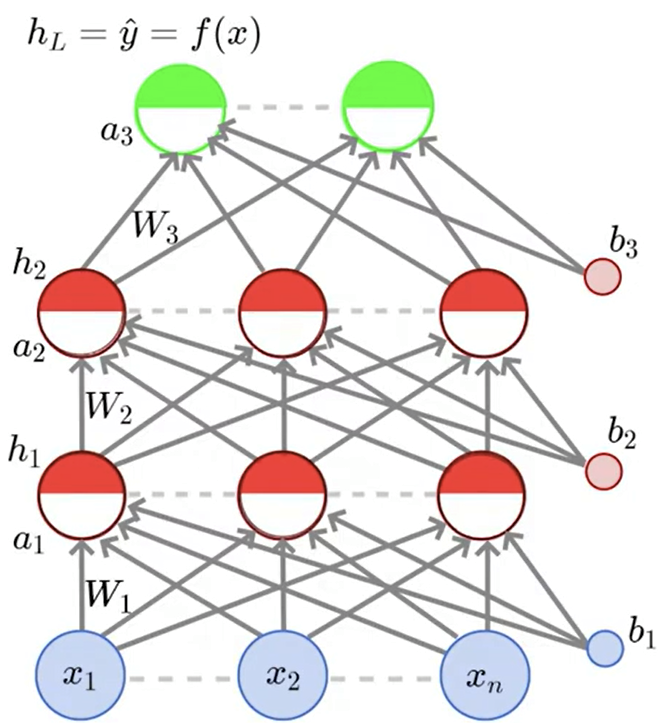
\includegraphics[width=0.5\linewidth]{Degree//static/DL_Feedforward_network.png}
        \caption{Feed Forward Network}
        \label{fig:DL-feedforward-network}
    \end{figure}
\end{itemize}

\subsection{Output functions and Loss functions}
\begin{itemize}
    \item Assume we are trying to predict values in the range of all real values, an appropriate loss function would be mean squared error function.
    \begin{equation*}
        \mathcal{L}(\theta)=\frac{1}{N}\sum_{i=1}^N\sum_{j=1}^k(\hat{y}_{ij}-y_{ij})^2
    \end{equation*}
    \item If we want to predict values in the range of real values, regression, then we can take the output function as a linear function
    \begin{equation*}
        f(x)=h_L=O(a_L)=W_Oa_L+b_O
    \end{equation*}
    \item Given that we are performing classification, then we can use cross entropy loss function. This is known as negative log likelihood function.
    \begin{equation*}
        -\frac{1}{N}\sum_{i=1}^N\sum_{j=1}^k(y_{ij}log(\hat{y}_{ij}) + (1-y_{ij})log(1-\hat{y}_{ij}))
    \end{equation*}
    \item Ensure that $\hat{y}$ is a probability distribution, one appropriate output function can be the softmax function
    \begin{equation*}
        \hat{y}_j=O(a_L)_j=\frac{e^{a_{L,j}}}{\sum_{i=1}^kw^{a_{L,i}}}
    \end{equation*}
    \begin{table}[H]
        \centering
        \begin{tabular}{|c|c|c|}
            \hline
             & Real Values & Probabilities \\
             \hline
            Output Activation & Linear & Softmax\\
            \hline
            Loss Function & Squared Error & Cross Entropy\\
            \hline
        \end{tabular}
        \caption{Choice of Output and Loss functions based on type of Output}
    \end{table}
\end{itemize}
\pagebreak

\subsection{Backpropagation}
\begin{itemize}
    \item Intuitively it can be written as
    \begin{figure}[H]
        \centering
        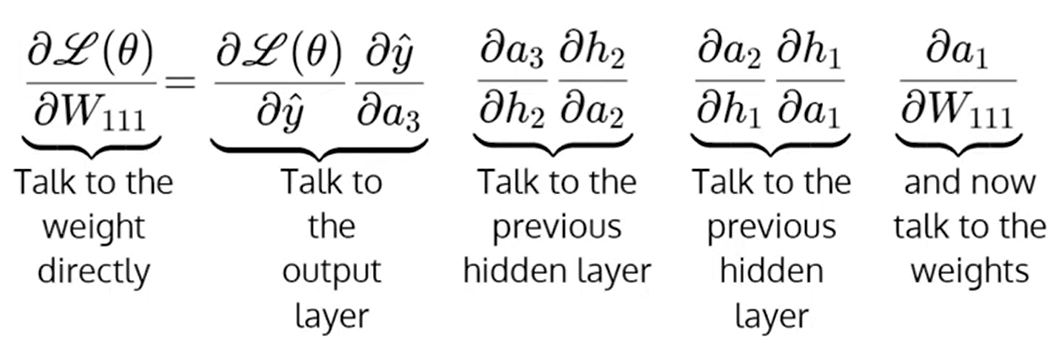
\includegraphics[width=0.5\linewidth]{Degree//static/DL_backprop_intuitie.png}
        \caption{Backpropagation Intuition}
        \label{fig:DL-backprop-intuition}
    \end{figure}
    \item For further discussion, the output function is considered to be softmax and the loss function is considered to be cross entropy.
    \item \textbf{Gradient w.r.t output layer}: We start with the part "Talk to the output layer".
    \begin{equation*}
        \mathcal{L}(\theta) = -\log{\hat{y}_l}\text{ }(l=\text{ true class label})
    \end{equation*}
    \begin{equation*}
        \frac{\partial}{\partial \hat{y}_i}\mathcal{L}(\theta)=\begin{cases}
            -\frac{1}{\hat{y}_l},\text{ if }i=l\\
            0,\text{ otherwise}
        \end{cases}=[0,...,0,-\frac{1}{\hat{y}_l},0,...,0]^T=-\frac{1}{\hat{y}_l}e_l
    \end{equation*}
    $e_l$is a $k-$dimensional vector whose $l^{th}$ element is $1$ and rest are $0$.
    \begin{equation*}
        \frac{\partial \mathcal{L}(\theta)}{\partial a_{L,i}}=-\frac{1}{\hat{y}_l}\frac{\partial \hat{y_l}}{\partial a_{L,i}}
    \end{equation*}
    Since, $\hat{y}_l$ is calculated using cross entropy it is dependent on all $a_L,i$
    \begin{equation*}
        \hat{y}_j=\frac{e^{a_{Lj}}}{\sum_ie^{a_{Li}}}
    \end{equation*}
    \begin{equation*}
        \frac{\partial \hat{y}_l}{\partial a_{L,i}}=\begin{cases}
            \hat{y}_l(1-\hat{y}_l),\text{ if }i= l\\
            -\hat{y}_l\hat{y}_i,\text{ if }i\neq l
        \end{cases}
    \end{equation*}
    We can now write the entire derivative in one shot as
    \begin{equation*}
        \frac{\partial \mathcal{L}(\theta)}{\partial a_{L,i}}=-\frac{1}{\hat{y}_l}(\hat{y}_l)(1_{l=i}-\hat{y}_i)=-(e_l-\hat{y})
    \end{equation*}
    \item \textbf{Chain rule among multiple paths}: If a function $p(z)$ can be written as a function of intermediate results $q_i(z)$ then we have
    \begin{equation*}
        \frac{\partial p(z)}{\partial z}=\sum_m\frac{\partial p(z)}{\partial q_m}\frac{\partial q_m}{\partial z}
    \end{equation*}
    \item \textbf{Gradient w.r.t hidden units}: Now we "Talk to the hidden layers", in this case $p(z)$ is the loss function, $z=h_{ij}$ and $q_m(z)=a_{Lm}$. We have
    \begin{equation*}
        \frac{\partial \mathcal{L}(\theta)}{\partial h_{ij}}=\sum_{m=1}^k\frac{\mathcal{L}(\theta)}{\partial a_{i+1,m}}W_{i+1,m,j}
    \end{equation*}
    \begin{equation*}
        \frac{\partial \mathcal{L}(\theta)}{\partial a_{ij}}=\frac{\partial \mathcal{L}(\theta)}{\partial h_{ij}}\frac{\partial h_{ij}}{\partial a_{ij}}=\frac{\partial \mathcal{L}(\theta)}{\partial h_{ij}}g'(a_{ij})
    \end{equation*}
    \item \textbf{Gradient w.r.t Parameters}: Finally, we "talk to the weights"
    \begin{equation*}
        \frac{\partial \mathcal{L}(\theta)}{\partial W_{kij}}=\frac{\partial \mathcal{L}(\theta)}{\partial a_{ki}}\frac{\partial a_{ki}}{\partial W_{kij}}=\frac{\partial \mathcal{L}(\theta)}{\partial a_{ki}}h^T_{k-1,j}
    \end{equation*}
    \begin{equation*}
        \frac{\partial \mathcal{L}(\theta)}{\partial b_{ki}}=\frac{\partial \mathcal{L}(\theta)}{\partial a_{ki}}\frac{\partial a_{ki}}{\partial b_{ki}}=\frac{\partial \mathcal{L}(\theta)}{\partial a_{ki}}
    \end{equation*}
    \item We can now write the full pseudocode as
    \begin{algorithm}[H]
        \caption{Forward Propagation}\label{alg:DL-forward-pass}
        \begin{algorithmic}[1]
            \For{$k=1$ to $L-1$}
                \State $a_k$ = $b_k+W_kh_{k-1}$
                \State $h_k$ = $g(a_k)$
            \EndFor
            \State $a_L$ = $b_L+W_Lh_{L-1}$
            \State $\hat{y}$ = $O(a_L)$
        \end{algorithmic}
    \end{algorithm}
    \begin{algorithm}[H]
        \caption{Backward Propagation}\label{alg:DL-backward-pass}
        \begin{algorithmic}[1]
            \State $\nabla_{a_L}\mathcal{L}(\theta)=-(e(y)-\hat{y})$
            \For{$k=L-1$ to $1$}
                \State $\nabla_{W_k}\mathcal{L}(\theta)$ = $\nabla_{a_k}\mathcal{L}(\theta)h_{k-1}^T$
                \State $\nabla_{b_k}\mathcal{L}(\theta)$ = $\nabla_{a_k}\mathcal{L}(\theta)$
                \State $\nabla_{h_{k-1}}\mathcal{L}(\theta)=W_k^T\nabla_{a_k}\mathcal{L}(\theta)$
                \State $\nabla_{a_{k-1}}\mathcal{L}(\theta)=\nabla_{h_{k-1}}\mathcal{L}(\theta)\odot [...,g'(a_{k-1,j}),...]$
            \EndFor
        \end{algorithmic}
    \end{algorithm}
    \item $g'$ for logistic function $\sigma(z)$ is $g(z)(1-g(z))$ and for tanh function is $1-(g(z))^2$.
    \item On flat surfaces, gradient descent moves very slow. How do we solve this?
\end{itemize}

\section{Gradient Descent Types}
\subsection{Momentum based Gradient Descent}
\begin{itemize}
    \item \textbf{Intuition}: If I am repeatedly being asked to move in the same direction then I should probably gain some confidence and start taking bigger steps in that direction. Just as a ball gains momentum while rolling down a slope.
    \item Update rule for momentum based gradient descent is
    \begin{equation*}
        \begin{split}
            &u_t=\beta u_{t-1}+\nabla w_t,\hspace{1cm}u_0=\nabla w_0,\text{ }u_{-1}=0\\
            &w_{t+1}=w_t-\eta u_t
        \end{split}
    \end{equation*}
    \item We are not only considering the current gradient, but we are also giving some importance to past history. $\beta$ is typically less than 1, so we give decreasing importance to previous histories. We have
    \begin{equation*}
        u_t = \beta u_{t-1}+\nabla w_t = \beta^2u_{t-2}+\beta \nabla w_{t-1}+\nabla w_t = ... = \sum_{\tau=0}^t\beta^{t-\tau}\nabla w_\tau
    \end{equation*}
    \item In addition to current update, also look at the history of updates.
    \item Even in the regions having gentle slopes, momentum based gradient descent is able to take large steps because the momentum carries it along.
    \item However, there is a possibility of overshooting our goal. This overshoot could lead to oscillations as well.
    \item Despite these oscillations, it will converge faster than gradient descent.
\end{itemize}

\subsection{Nesterov Accelerated Gradient Descent}
\begin{itemize}
    \item Can we do something to reduce the oscillations observed in momentum based gradient descent?
    \item \textbf{Intuition}: Look before you leap, we ask the weights to move by two parts $\beta u_{t-1}$ and $\nabla w_t$. The idea is to first move by $\beta u_{t-1}$ and then compute $\nabla w_t$. So instead of relying only on current gradient we are essentially "looking ahead" and computing new gradient.
    \item Update rule for NAG is
    \begin{equation*}
        \begin{split}
            &u_t = \beta u_{t-1} + \nabla (w_t-\beta u_{t-1})\\
            &w_{t+1} = w_t - \eta u_t\\
            &\text{with }u_{-1}=0,\text{ and }0\leq \beta \leq 1
        \end{split}
    \end{equation*}
\end{itemize}

\subsection{Stochastic vs Batch Gradient Descent}
\begin{itemize}
    \item Regular gradient descent goes over the entire data once before updating the parameters. Because this is the true gradient of the loss as derived earlier. Hence, theoretical guarantees hold.
    \item Imagine we have a million points in the training data, then it will take very long.
    \item In \textbf{stochastic} version, we update the parameters for every point in the data. Now if we have a million data points then we will make a million updates in each epoch.
    \item However, this is an approximate gradient. Hence, we have no guarantee that each step will decrease the loss.
    \item So, going over a large data once is bad, going over a single point and updating is bad, but going over some data points and updating is ok.
    \item This is the idea for \textbf{mini-batch} gradient descent.
    \item 1 epoch is one pass over the entire data, 1 step is one update of the parameters, $N$ is the number of data points, and $B$ is the mini batch size.
    \item So, for regular gradient descent the number of epochs is the same as number of steps, for stochastic gradient descent the number of steps is the same as $N$, and for mini-batch gradient descent the number of steps is the same as $\frac{N}{B}$.
    \item It is intuitive that a larger batch size is better, but we sacrifice on time.
    \begin{table}[H]
        \centering
        \begin{tabular}{|c|c|}
            \hline
            \textbf{Algorithm} & \textbf{\# of steps in 1 epoch}\\
            \hline
            Vanilla (Batch) Gradient Descent & 1 \\
            \hline
            Stochastic Gradient Descent & $N$\\
            \hline
            Mini Batch Gradient Descent & $\frac{N}{B}$\\
            \hline
        \end{tabular}
        \caption{Stochastic vs Mini Batch Gradient Descent}
        \label{tab:DL-stochastic-vs-mini-batch}
    \end{table}
\end{itemize}

\subsection{Scheduling Learning Rate}
\begin{itemize}
    \item Instead of using momentum and NAG we could have simply increased the learning rate, but on regions which have a steep slope, the already large gradient would blow up farther.
    \item What we need is for the learning rate to be small when gradient is high and vice versa.
    \item Tune learning rate, try different values on a log scale: $0.0001, 0.001, 0.001, 0.1, 1.0$.
    \item Run a few epochs with each of these and figure out a learning rate which works best. Now do a finer search around this value.
    \item These are just heuristics, no clear winning strategy.
    \item \textbf{Annealing learning rate}: Decrease the learning rate as we get close to the minima.
    \item \textbf{Step Decay}: Halve the learning rate after every 5 epochs or halve the learning rate after an epoch if the validation error is more than what it was at the end of the previous epoch.
    \item \textbf{Exponential Decay}: $\eta = \eta_0^{-kt}$, where $\eta_0$ and $k$ are hyperparameters and $t$ is a step number. However, choosing $k$ becomes complex.
    \item \textbf{1/t Decay}: $\eta = \frac{\eta_0}{1+kt}$, again choosing $k$ is a bit tricky, ideally we won't use these learning rates.
    \item For momentum the following schedule was suggested by Sutskever et al., 2013
    \begin{equation*}
        \beta_t = min(1-2^{-1-\log_2{(\lfloor \frac{t}{250}\rfloor+1})},\beta_{max})
    \end{equation*}
    $\beta_{max}$ is chosen from $\{0.999,0.995,0.99,0.9,0\}$
    \item In practice, often a line search is done to find a relatively better value of $\eta$. Update $w$ using different values of $\eta$ then pick the best $w$ based on loss function.
\end{itemize}

%\section{Gradient Descent with Adaptive Learning Rates}

\end{document}